\documentclass[11pt]{article}
\usepackage{graphicx}
\usepackage{hyperref}
\begin{document}

\title{Crazyflie Manual}
\author{Jianxin Sun}
\date{3/9/2014}
\maketitle

\section{Fast setup}
\subsection{Setup Virtual Machine}
\begin{itemize}
\item Go to 

\url{https://www.virtualbox.org/}
\item Click Downloads on the right
\item Download ``VirtualBox platform packages'' and ``VirtualBox 4.3.14 Oracle VM VirtualBox Extension Pack''
\item Install the ``VirtualBox platform packages (version no.)''
\item Install the ``VirtualBox (version no.) Oracle VM VirtualBox Extension Pack''
\item Go to 

\url{http://wiki.bitcraze.se/projects:virtualmachine:index}
\item Download the newest Bitcraze VM file
\item Open VirtualBox
\item Import the downloaded Bitcraze VM file into VirtualBox (In mac, one can drag and drop the file into the VirtualBox window)
\item Now you should see a bar showing the process of importing the Bitcraze VM file
\item Once finished, a Bitcraze virtual machine should appear in the right side of VirtualBox software
\item Launch the virtual machine. 

User name: bitcraze

Password: crazyflie
\end{itemize}

\subsection{Connect to Crazyflie Using PC client}
\begin{itemize}
\item Once the virtual machine is launched, you should see a Xubuntu desktop fig. \ref{fig:desktop}. If blackscreen, use left win + F to enter fullscreen mode. In full screen mode, if desktop appears, use left win + F to exit fullscreen; if not, relaunch the virtual machine
\item There is no need to upgrade anything, double click the ``Crazyflie PC client latest'' icon on desktop. The client gui should launch as in fig. \ref{fig:pcgui}
\item Now plug in the radio dongle provided by Crazyflie into your PC's usb port
\item Enable the radio device in virtual machine by selecting it as shown in fig. \ref{fig:radiousb}
\item Connect you PS3/PS4/Xbox360 controller to mac, enable it in virtual machine just as you enable radio. Make sure that thrust input is 0
\item Turn on your mini quad, check section Flight for detail
\item Now in PC client GUI, click the Connect button, it should start scan for mini quad
\item If your mini quad is on with red led blinking at 2 Hz, you should see it in the list
\item If your mini quad is on with red led blinking at 2 Hz and it's not in the list, click scan button again
\item If your mini quad's red led is not blinking at 2 Hz, go to section Troubleshoot 
\item Once you see the quad appear in the list as fig. \ref{fig:radioconnect}, make sure you hold the quad firm in hand and the propellers have clear space to spin, click the connect button
\item Now if everything is normal, you should see the data obtained fig. \ref{fig:connectedquad}
\item Now to fly it, go to section Flight.
\item To disconnect, click the disconnect button on top
\end{itemize}



\section{Ubuntu setup}
To install the PC client on Ubuntu, follow the following link: 

\url{http://wiki.bitcraze.se/projects:crazyflie:pc\_utils:install}


\section{Flight}
\subsection{Before Flight}
\begin{itemize}
\item read the User Guide: 

\url{http://wiki.bitcraze.se/projects:crazyflie:userguide:index}

This covers the basic concepts such as the meaning of led lights, how to turn on the mini quad, how to find out the front direction of the mini quad, etc.
\item check your input device: 

\url{http://wiki.bitcraze.se/projects:crazyflie:pc\_utils:inputdevices}
\item Make sure you take necessary safety measures: 

\url{http://wiki.bitcraze.se/projects:crazyflie:safety}
\end{itemize}

\subsection{Pre-Flight test}
\begin{itemize}
\item You should have connected your mini quad to your PC client right now and getting the live feedback
\item You should also have connected your controller to your PC and it is recognized by the PC client
\item Now you should fix the mini quad to ground while ensure there are clear space for propellers to rotate.
\item Test each stick of your controller to ensure that the control mapping is alright.
\item If everything is alright, go to next step
\end{itemize}

\subsection{Fly it}
Controlling the mini quad can be difficult at first as it is very agile. 
One need to practice it a lot to master it. Practice it inside the web area of the lab. 
Increase the thrust very gently and try not to fly too high above ground as crashes are inevitable in the first few flights.
When landing, try to decrease the height slowly.
When changing pitch/roll angles, remember to adjust thrust accordingly as part of the thrust will be used to move the quad forward/sideways.

\section{Troubleshoot}
\subsection{regular problems}
Check these two pages:

\url{http://wiki.bitcraze.se/projects:crazyflie:faq}

\url{http://wiki.bitcraze.se/projects:crazyflie:userguide:troubleshooting}

\section{API usage}
Some basic info are provided in: 

\url{http://wiki.bitcraze.se/projects:crazyflie:pc\_utils:pylib}

Your controller should be a multi thread program that based on callback functions. The basiclog.py and basicparam.py in example folder demonstrate how to use callback functions to retrieve data from mini quad. The ramp.py shows how to start a thread that takes care of sending control inputs. Make sure you understand these examples before writing your own code.

To run the provided examples that retrieve data, set parameter, control motor, and scan available quad, see the following instruction:

\begin{itemize}
\item connect radio to PC and turn on your mini quad
\item open up a terminal
\item cd to the cfclient project folder, in the virtual machine setup, use this command:

	cd ~/projects/crazyflie-clients-python/examples/
\item to receive flight data, run:

	python basiclog.py
\item to receive the param list, run:

	python basicparam.py
	
	Remark: the source code of this example has some issues:
	
	To make it work, uncomment ``line 174'' and comment ``line 175''.
	
	Also remember that this program changes the parameter in your quad. So remember to change it back before flying it. A little change in ``line 128'' should work.
	
	
\item to control the motors, ensure that quad is fixed to ground and the propellers are free to move, run:
	
	python ramp.py
\item to scan for available quad, run:

	python scan.py
\end{itemize}

These four example programs demonstrate basic idea of how to get feedback and send out control signal. With these two, one should be able to develop a feedback control loop.

Source code can also be found in: 

\url{https://github.com/bitcraze}

The following links explain some basic ideas about synchronizing between threads, which should be helpful when writing the control loop, as both the control thread and the logging thread will attempt to retrieve/update current flight data. The idea here is to encapsulate the flight data into a class that can only be accessed/modified by one thread at a time, thus preventing the control thread and logging thread from interfering each other.

\url{http://effbot.org/zone/thread-synchronization.htm}

\url{https://docs.python.org/3/library/concurrency.html}

Here is a sample code written by Jianxin Sun, for the purpose of building a basic control loop:

\url{https://github.com/JXS2012/CrazyflieHover}

Remark:

To obtain parameter and log toc, use the PC client gui interface: click view$\rightarrow$tabs$\rightarrow$log toc(parameter)


\newpage
\section{Improve performance}
Due to the limit of data transmit rate, one can only grab limited sensor info from the quad, which is often insufficient for achieving better control over the quad. A possible improvement is to add your feature into the existing quad firmware, allowing access to onboard sensors at a much higher rate. However rewrite the firmware could be a challenging process since only source codes are available. To start, one can go to the following link to study how they write the ``stabilizerAltHoldUpdate'' function in their firmware:

\url{https://github.com/bitcraze/crazyflie-firmware/blob/master/modules/src/stabilizer.c}

And there are multiple ways of improving the code, say implementing a Kalman Filter to get better velocity estimate.

\begin{figure}[h]
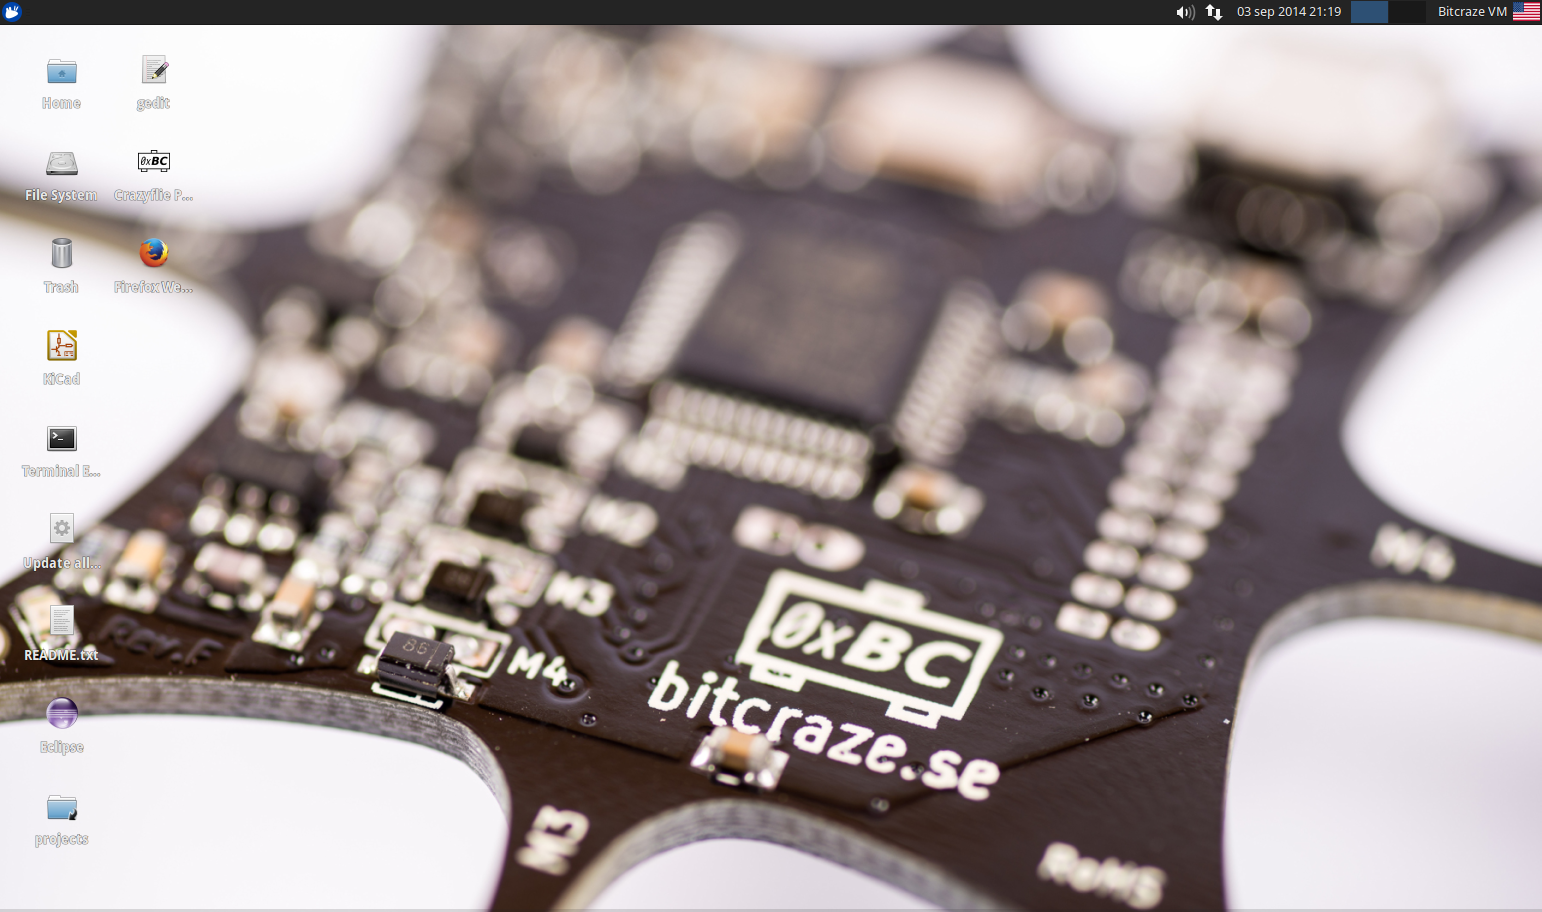
\includegraphics[width=\linewidth]{desktop.png}
\caption{Xubuntu Desktop}
\label{fig:desktop}
\end{figure}

\begin{figure}[h]
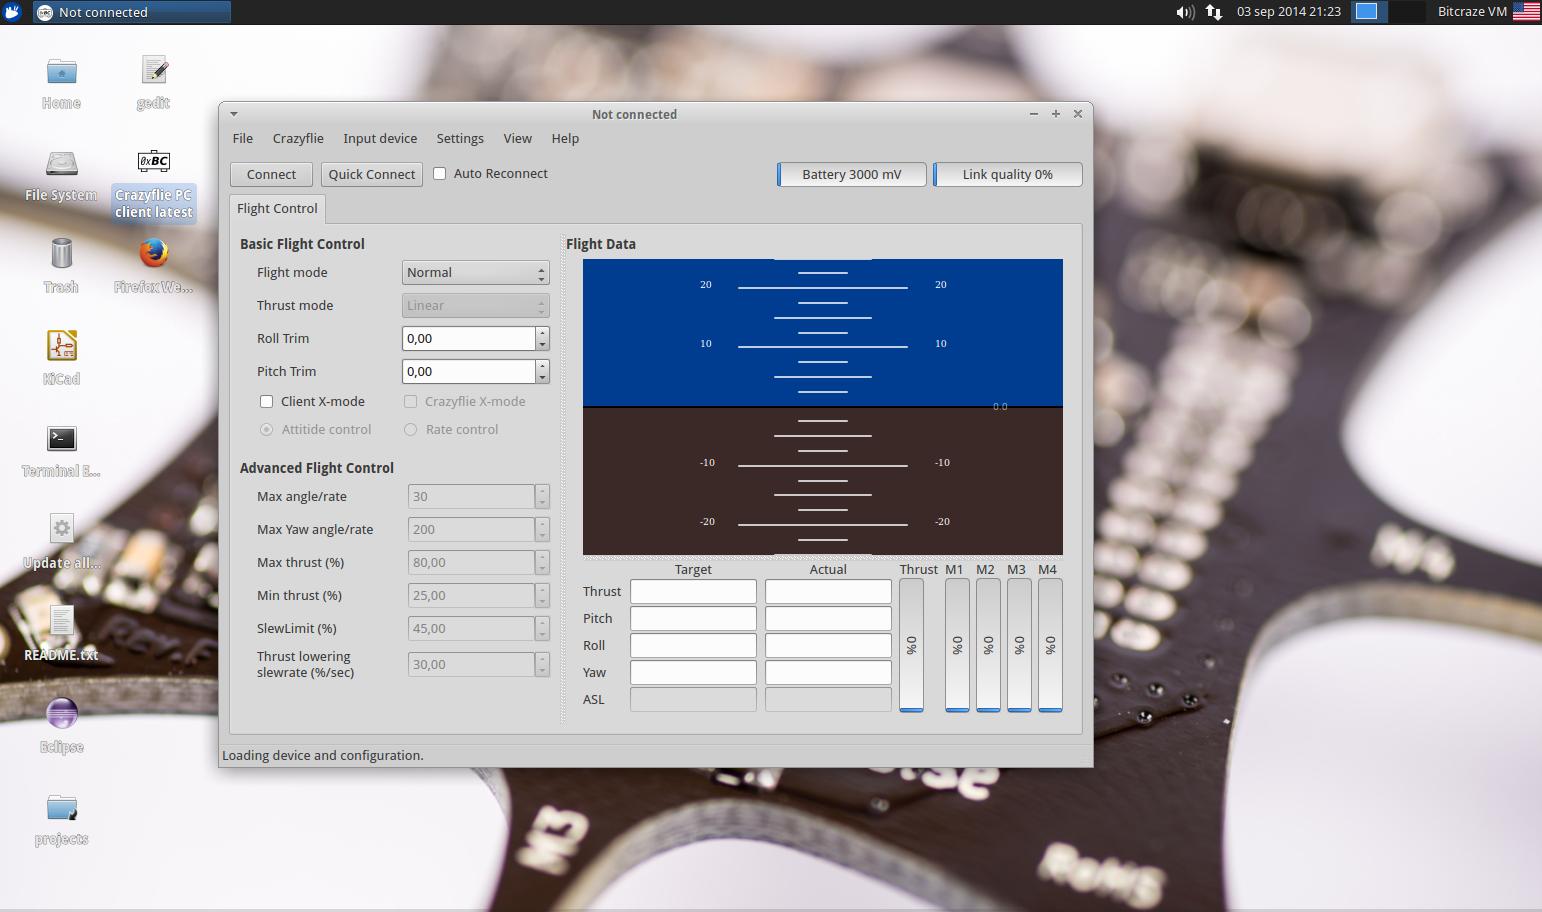
\includegraphics[width=\linewidth]{pcgui.png}
\caption{Crazeflie PC client}
\label{fig:pcgui}
\end{figure}

\begin{figure}[h]
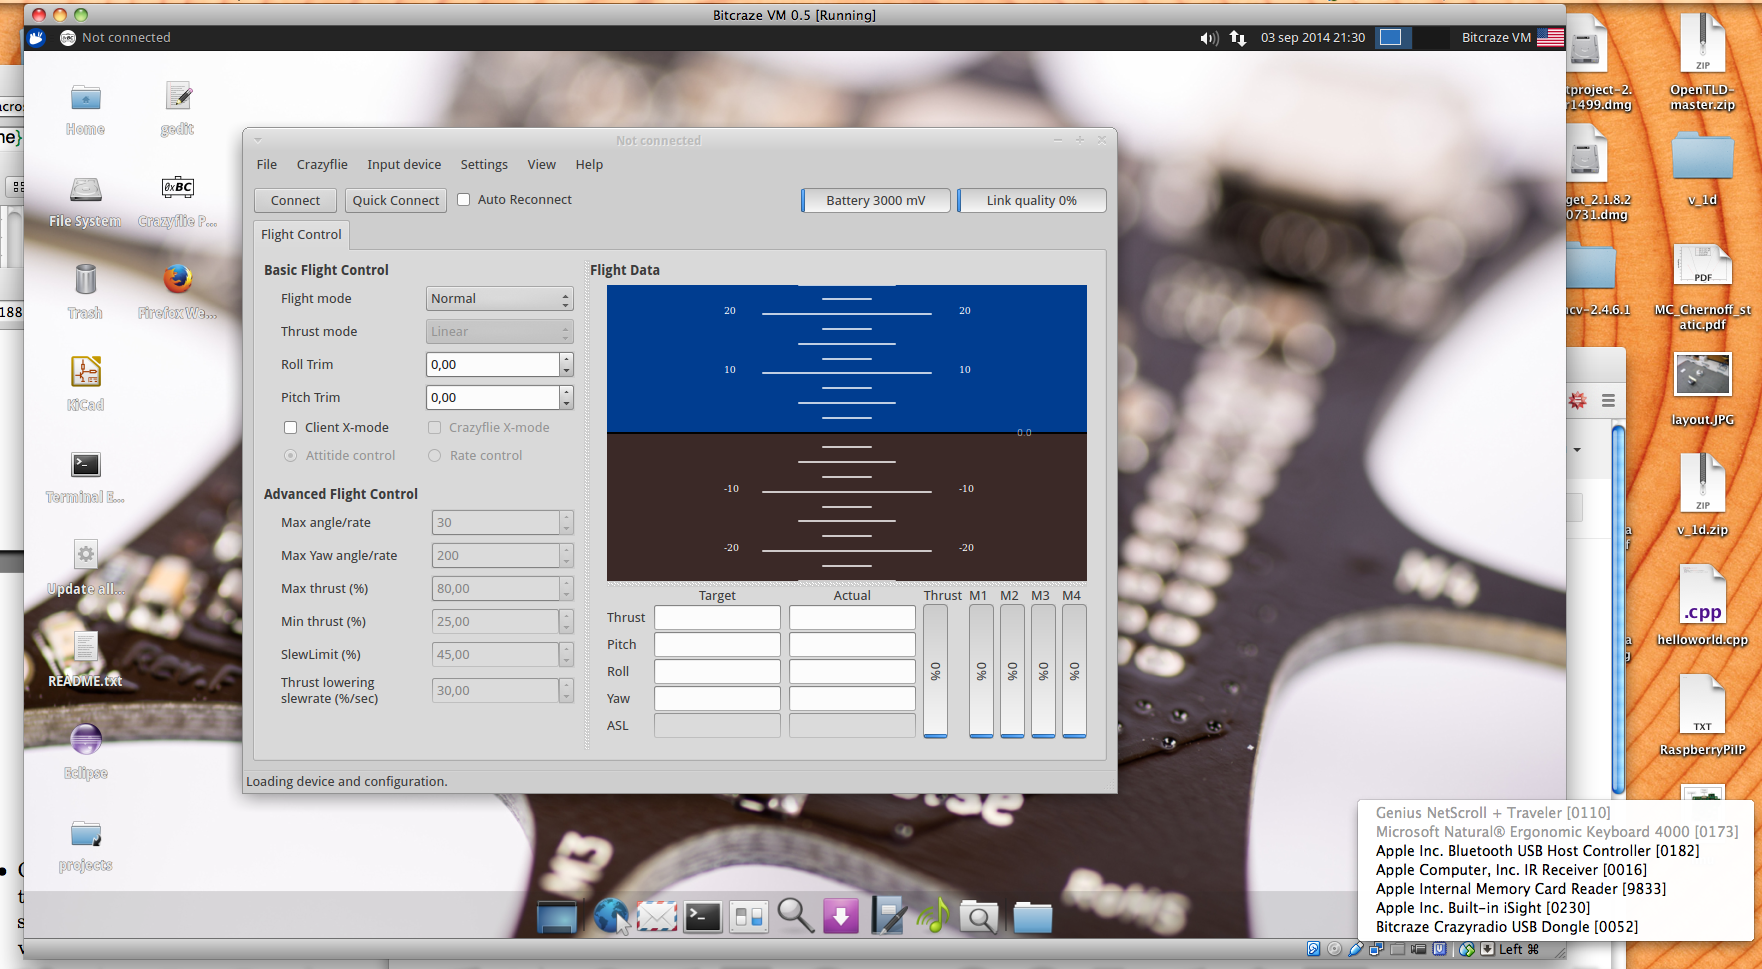
\includegraphics[width=\linewidth]{radiousb.png}
\caption{Enable the Bitcraze raido by clicking the usb icon in the bottom of virtual machine window and click the Bitcraze device}
\label{fig:radiousb}
\end{figure}

\begin{figure}[h]
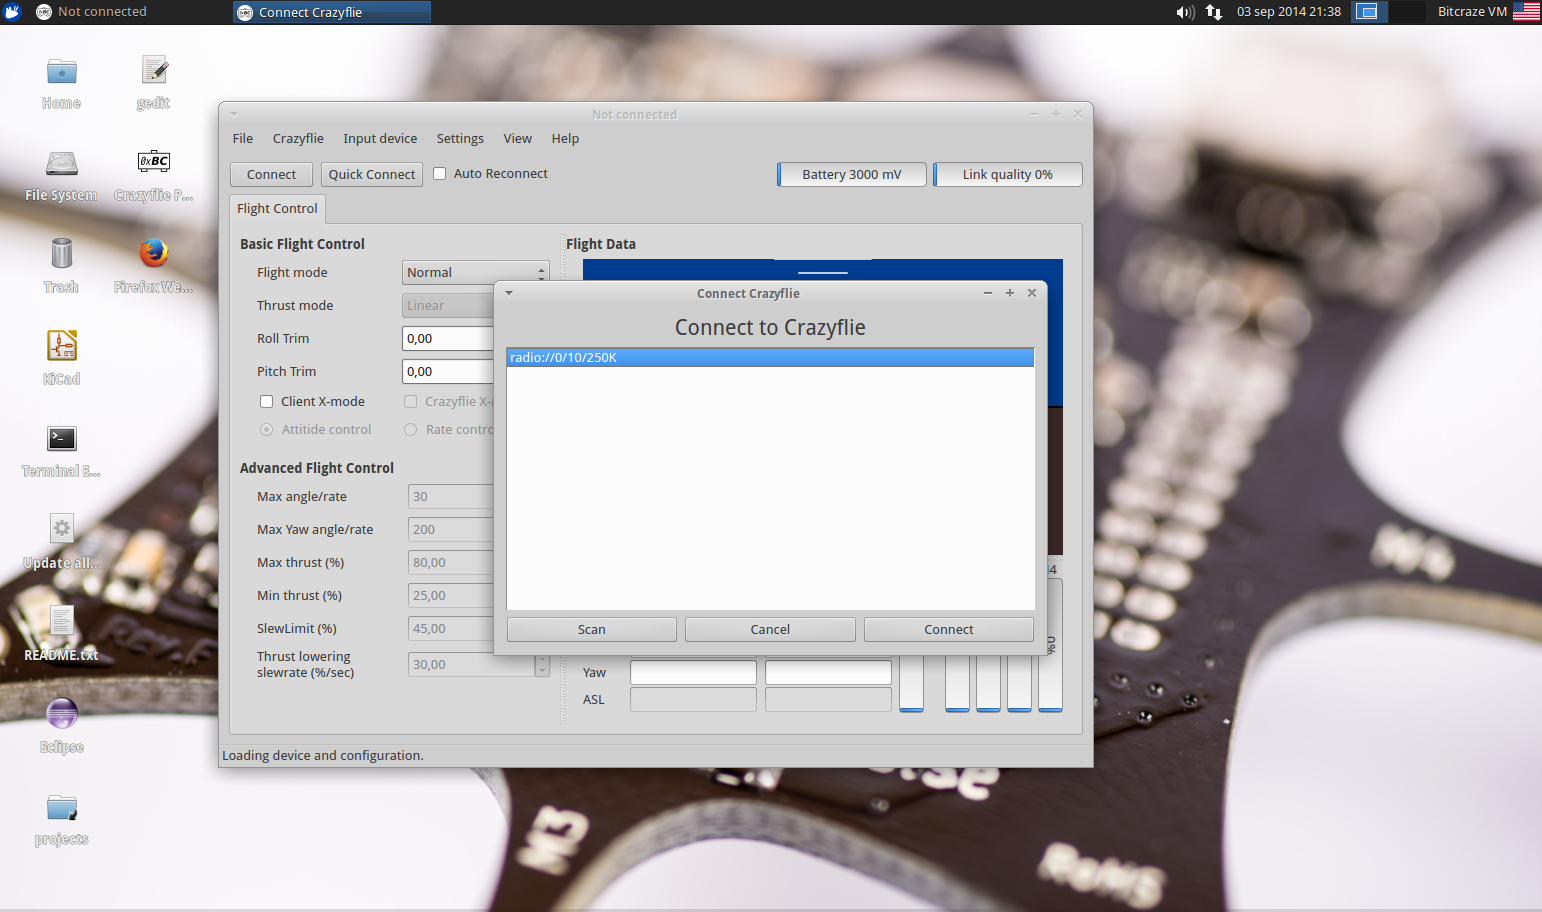
\includegraphics[width=\linewidth]{radioconnect.png}
\caption{Now the radio://0/10/250K is the quad currently available}
\label{fig:radioconnect}
\end{figure}

\begin{figure}[h]
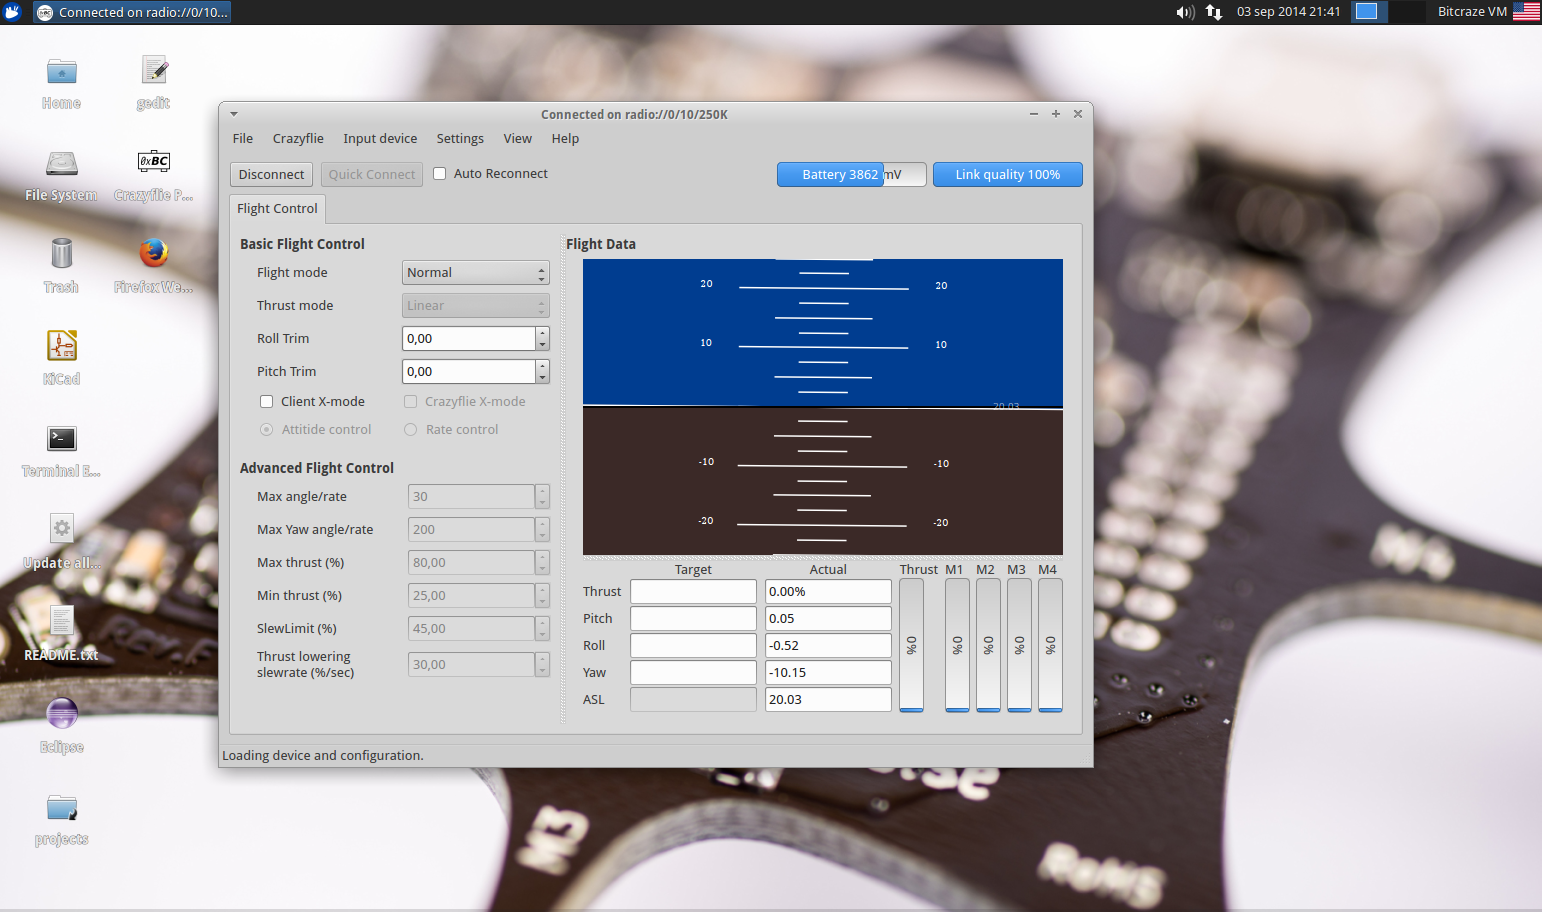
\includegraphics[width=\linewidth]{connectedquad.png}
\caption{Real time data received from mini quad}
\label{fig:connectedquad}
\end{figure}

\end{document}
